% !TeX spellcheck = cs_CZ
\wikitextrule
\begin{example}\label{mai:exam069}
  \textbf{Normální rozdělení}\newline\small
  Veličinou s normálním rozdělením rozumíme takovou náhodnou veličinu X, jejíž hustota 
  pravděpodobnosti má tvar
  \adjustbox{minipage=[c][33pt][c]{406pt}}{%
    \begin{equation}\label{mai:eq069}
      w(x) = \dfrac{1}{\sigma\sqrt{2\pi}}\exp\left(-\dfrac{(x-x_0)^2}{2\sigma^2}\right),
             \qquad x\in(-\infty, \infty).
    \end{equation}
  }
  Grafem této funkce je \textbf{Gaussova křivka}. Distribuční funkce má tvar
  \adjustbox{minipage=[c][35pt][c]{406pt}}{%
    \begin{equation}\label{mai:eq70}
      F(x) = \int_{-\infty}^{x}\dfrac{1}{\sigma\sqrt{2\pi}}
               \exp\left[-\dfrac{(x-x_0)^2}{2\sigma^2}\right]\dd{x}.
    \end{equation}
  }
  Přitom \(F(\infty) = 1\) (pravděpodobnost jistého jevu). Skutečně, platí
  \begin{equation*}
    \int_{-\infty}^{\infty}\dfrac{1}{\sigma\sqrt{2\pi}}
           \exp\left[-\dfrac{(x-x_0)^2}{2\sigma^2}\right]\dd{x}
    = \dfrac{\sigma\sqrt{2}}{\sigma\sqrt{2\pi}}
      \int_{-\infty}^{\infty}\exp\left(-t^2\right)\dd{t}
    =1.
  \end{equation*}
  Takzvaný Laplaceův integrál \(\int_{-\infty}^{\infty}\exp(-t^2)\dd{t} = \sqrt{\pi}\) 
  sice můžeme najít v tabulkách a v dalším dílu jej i odvodíme, v tu to chvíli se však budeme řídit 
  výrokem lorda Kelvina: „Matematik je ten, komu je toto zřejmé jako je zřejmé vám, že dvakrát dvě 
  jsou čtyři.“ Příklady normálního rozdělení pro různé hodnoty \(\sigma\) a odpovídající 
  distribuční funkce vidíme na obrázku \ref{mai:fig046} a \ref{mai:fig047}.

  {\centering
    \captionsetup{type=figure}
    \begin{tabular}{cc}
     \subfloat[ ]{\label{mai:fig046a}
       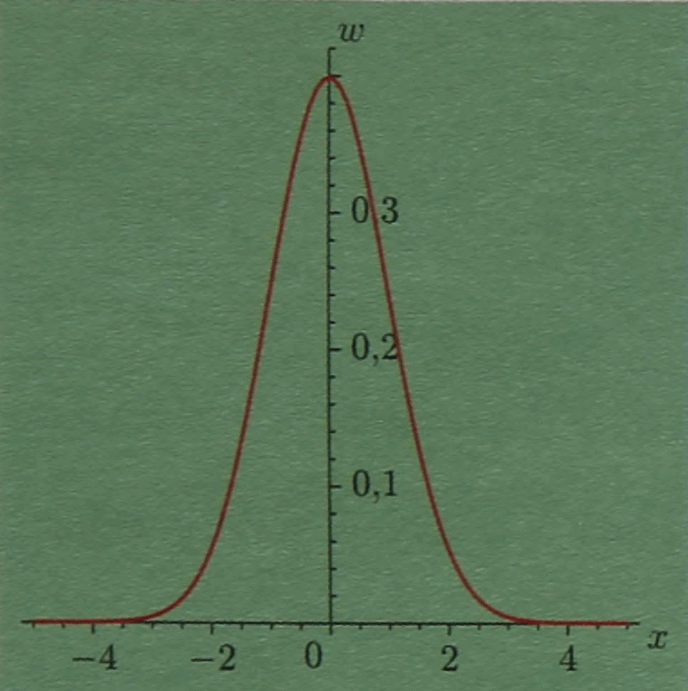
\includegraphics[width=0.35\linewidth]{mai_fig046a.png}}              &
%     \hspace{1pt}
     \subfloat[ ]{\label{mai:fig046b}
       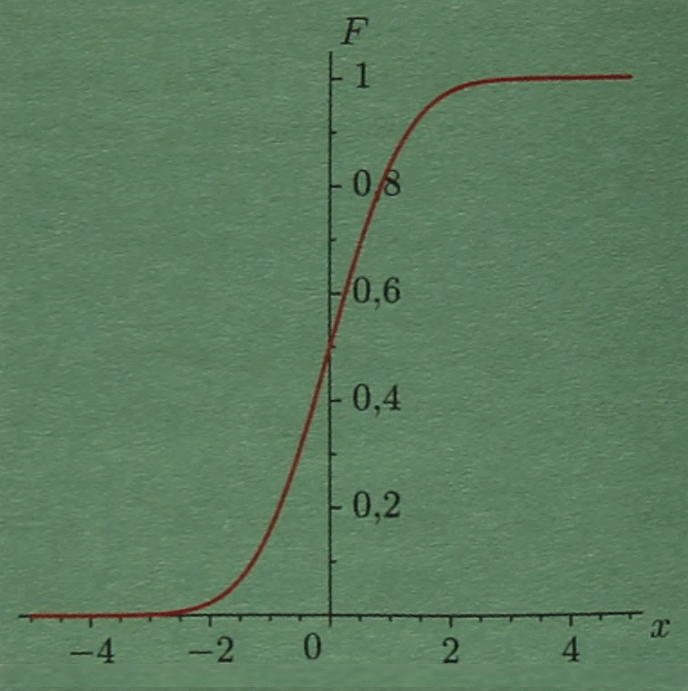
\includegraphics[width=0.35\linewidth]{mai_fig046b.png}}
%     \hspace{1pt}
    \end{tabular}
    \captionof{figure}{Normální rozdělení a jeho distribuční funkce pro \(\sigma(x) = 1\) a \(X_0 = 
               0\) \cite[s.~240]{Musilova2009MA1}}
    \label{mai:fig046}
  \par}
  
  Určíme střední hodnotu a rozptyl veličin s tímto rozdělením:
  \begin{align*}
    \langle x \rangle 
      &= \int_{-\infty}^{x}\dfrac{1}{\sigma\sqrt{2\pi}}x\cdot
         \exp\left[-\dfrac{(x-x_0)^2}{2\sigma^2}\right]\dd{x}.  
       = \dfrac{\sigma\sqrt{2}}{\sigma\sqrt{2\pi}}
         \int_{-\infty}^{\infty}\left(x_0+t\sigma\sqrt{2}\right)\cdot\exp\left(-t^2\right)\dd{t}  \\
      &= \dfrac{x_0}{\sqrt{\pi}}\int_{-\infty}^{\infty}\exp\left(-t^2\right)\dd{t}
       + \dfrac{1}{\sqrt{\pi}}\int_{-\infty}^{\infty}t\sigma\sqrt{2}\cdot\exp\left(-t^2\right)\dd{t}
       =x_0.
  \end{align*}
  Druhý z integrálů je totiž roven nule, neboť integrand je lichá funkce.
  \begin{equation*}
    D(X) = \dfrac{1}{\sigma\sqrt{2\pi}}\int_{-\infty}^{\infty}\left(x - x_0\right)^2 
           \exp\left[-\dfrac{(x-x_0)^2}{2\sigma^2}\right]\dd{x}
         = \dfrac{2\sqrt{2}\sigma^3}{\sigma\sqrt{2\pi}}
           \int_{-\infty}^{\infty}t^2\exp\left(-t^2\right)\dd{t}
         = \sigma^2.
  \end{equation*}
  Integrál \(\int_{-\infty}^{\infty}t^2\exp\left(-t^2\right)\dd{t} = \frac{\sqrt{\pi}}{2}\) lze buď 
  opět najít v tabulkách, nebo jej metodou per partes převést na výpočet Laplaceova integrálu:
  \begin{equation*}
    I = \int_{-\infty}^{\infty}t\cdot t\exp\left(-t^2\right)\dd{t} 
      = \left[-\dfrac{t}{2}\exp\left(-t^2\right)\right]_{-\infty}^{\infty}
      + \dfrac{1}{2}\int_{-\infty}^{\infty}\exp\left(-t^2\right)\dd{t}.
  \end{equation*}

  {\centering
    \captionsetup{type=figure}
    \begin{tabular}{cc}
     \subfloat[ ]{\label{mai:fig047a}
       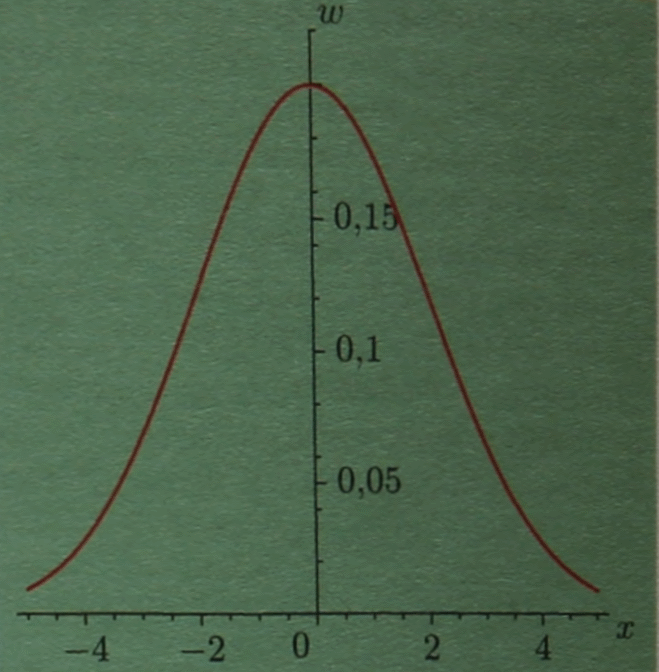
\includegraphics[width=0.35\linewidth]{mai_fig047a.png}}              &
%     \hspace{1pt}
     \subfloat[ ]{\label{mai:fig047b}
       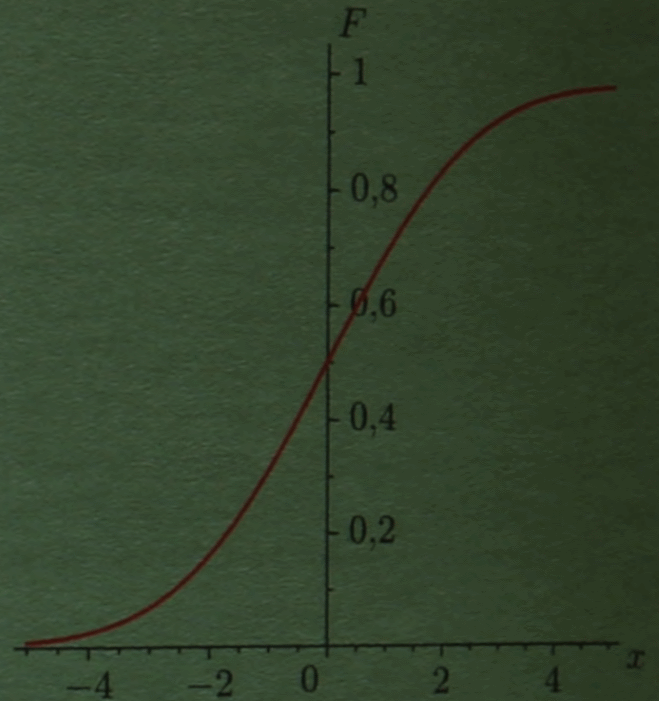
\includegraphics[width=0.35\linewidth]{mai_fig047b.png}}
%     \hspace{1pt}
    \end{tabular}
    \captionof{figure}{Normální rozdělení a jeho distribuční funkce pro \(\sigma(x) = 2\) a \(X_0 = 
               0\) \cite[s.~241]{Musilova2009MA1}}
    \label{mai:fig047}
  \par}
  
  Distribuční funkce normálního rozdělení, zvaná \(errorfunkce\), je běžnou součástí různých 
  počítačových programů, takže poměrně snadno zjistíme pravděpodobnostní obsah intervalu určeného 
  směrodatnou odchylkou \(\sigma(x) = \sqrt{d(X)} = \sigma\). Pravděpodobnost, že hodnota náhodné 
  veličiny \(X\) s normálním rozdělením leží v intervalu \((x_0 - \sigma, x_0 + \sigma)\), je 
  zhruba \SI{68.3}{\percent}. V souvislosti s normálním rozdělením se často užívají další 
  dva druhy odchylek. \textbf{Pravděpodobná chyba} \(\theta\) určuje interval \((x_0 - \theta, x_0 
  + \theta)\), v  němž leží hodnota veličiny \(X\) s pravděpodobností \SI{50}{\percent}. 
  \textbf{Krajní chyba} \(\kappa\) určuje interval \((x_0 - \kappa, x_0 + \kappa)\), v němž leží 
  hodnota veličiny \(X\) s pravděpodobností \SI{99.7}{\percent}. Z tabelovaných hodnot 
  \(errorfunkce\) zjistíme, že platí
  \begin{equation}\label{mai:eq71}
   \theta \simeq \dfrac{2}{3}\sigma, \qquad \kappa = 3\sigma
  \end{equation}
  Poznamenejme, že normálním rozdělením \(w(x)\) (\ref{mai:eq069}) lze přibližně nahradit 
  Bernoulliovo rozdělení
  \begin{equation*}
    w_{Ber}(x) = \begin{pmatrix} n \\ x \end{pmatrix}p^x(1 - p)^{n-x},\qquad
    \langle x \rangle = np, \qquad
    D(x) = np(1-p)
  \end{equation*}
  pro velké hodnoty \(n\) a také Poissonovo rozdělení
  \begin{equation*}
    w_{Pois}(x) = e^{-\langle x \rangle}\dfrac{\langle x \rangle^x}{x!}, \qquad 
    D(x) = \langle x \rangle
  \end{equation*}
  s velkou střední hodnotou \(\langle x \rangle\)
\normalsize
\end{example}